This section presents the MBT process, the CLARET notation, and the basic idea behind the two strategies used for reducing test case discard, distance functions, and machine learning.

\subsection{Model-Based Testing}
MBT aims to automatically generate and manage test suites from software specification models. MBT may use different model formats to perform its goals (e.g., Labeled Transition System (LTS) \citep{tretmans2008model}, UML diagrams \citep{bouquet2007subset}). As MBT test suites are derived from specification artifacts, their test cases tend to reflect the system behavior \citep{STVR:STVR456}. \citet{Utting:2006:PMT:1200168} discuss a series of benefits of using MBT, such as sound test cases, high fault detection rates, and test cost reduction. On the other hand, regarding MBT limitations, we can list the need for well-built models, huge test suites, and a great number of obsolete test cases during software evolution. 

Figure \ref{fig: mbt_flow} presents an overview of the MBT process. The system models are specified through a DSL (e.g., UML) and a test generation tool is used to create the test suite. However, as the system evolves, edits must be performed on its models to keep them up-to-date.  If any fault is found, the flow goes back to system development. These activities are repeated until the system is mature for release. Note that previous test suites are discarded, and important historical data may be lost in this process.

%On the left-hand side we can see the first test suite generation. However, as the system evolves, edits must be performed on its models to keep them up-to-date (right-hand side). Thus, a new test suite is generated, imported to a test management tool, and run. If any fault is found, the flow goes back to system development. These activities are repeated until the system is mature for release. Note that previous test suites are discarded and important historical data may be lost in this process.

\begin{figure}[h]
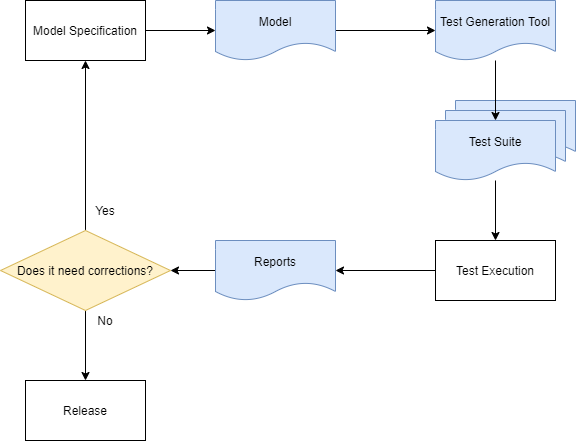
\includegraphics[width=.48\textwidth]{LaTeX/figs/MBT_FLOW_NEW.png}
\caption{MBT Process}
\label{fig: mbt_flow}
\end{figure}


\subsection{CLARET}
CLARET \citep{dalton2017claret,dalton2018mbtagile} is a DSL and tool that allows the creation of use case specifications using natural language. It was designed to be the central artifact for both requirement engineering and MBT practices in agile projects. Its toolset works as a syntax checker for use cases description files and provides visualization mechanisms for use case revision. Listing 1 presents a use case specification using CLARET.  

From the use case description in Listing 1, CLARET generates its equivalent Annotated Labeled Transition System (ALTS) model \citep{tretmans2008model} (Figure \ref{fig:alts}). Transition labels starting with \textit{[c]} indicate pre or post conditions, while the ones starting with \textit{[s]} and \textit{[e]} are regular and exception execution steps, respectively.

\begin{figure}[h!] 
\centering 
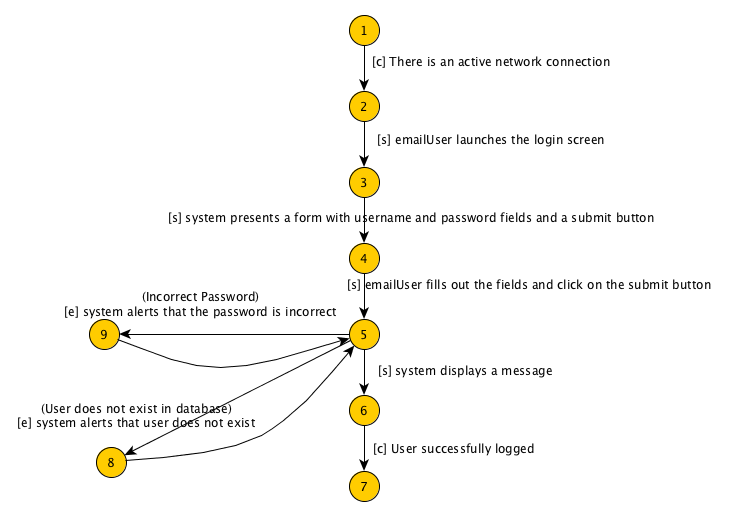
\includegraphics[width=.5\textwidth]{figs/UserLogin.png}
\caption{ALTS model of the use case from Listing 1.}
\label{fig:alts}
\end{figure}

CLARET's toolset includes a test generation tool, LTS-BT (Labeled Transition System-Based Testing) \citep{cartaxo2008lts}. LTS-BT is an MBT tool that uses as input LTS models and generates test suites by searching for valid graph paths. The generated tests are reported in XML files that can be directly imported to a test management tool, TestLink\footnote{http://testlink.org/}.
%Besides generation, it includes a series of algorithms for model-based test selection, reduction, and prioritization. 
The test cases reported in Section \ref{sec:motiv} were collected from LTS-BT.

\subsection{Distance Functions}

Distance functions are metrics for evaluating how similar, or different, are two strings \citep{coutinho2016analysis}. Distance functions have been used in different contexts (e.g., \citep{runkler2000automatic,okuda1976method,lubis2018combination}). For instance, \citet{coutinho2016analysis} use distance functions for reducing MBT suites. 

There are several distance functions (e.g., \citep{hamming1950error,han2007efficient:LCS,huang2008similaritycosine,de1mahalanobis:jaro,Levenshtein_SPD66}). For instance, the Levenshtein function \citep{Levenshtein_SPD66,kruskal1983overview} (equation described below) compares two strings (\textit{a} and \textit{b}) and calculates the number of required operations to transform \textit{a} into \textit{b}, and vice-versa; where $1_{ai \neq bj}$ is the indicator function equal to 0 when $a_{i} \neq b_{j}$ and equal to 1 otherwise, and $lev_{a,b}$ is the distance between the first $i$ characters of \textit{a} and the first $j$ characters of \textit{b}.

To illustrate its use, consider two strings \textit{a} = ``kitten'' and \textit{b} = ``sitting''. Their Levenshtein distance is three, since three operations are needed to transform a to b: (i) replacing `k' by `s'; (ii) replacing `e' by `i'; and (iii) inserting `g' at the end. A more detailed discussion about the Levenshtein and others functions, as well as an open-source implementation of them are available\footnote{https://github.com/luozhouyang/python-string-similarity}.


\resizebox{\columnwidth}{!}{
\begin{equation*}
   lev_{a,b}(i,j) = 
    \begin{cases}
    max(i,j)  \qquad \qquad \qquad \qquad \qquad \text{\textit{if min(i,j) = 0}}&\\
        min 
        \begin{cases}
            lev_{a,b}(i-1,j) + 1\\
            lev_{a,b}(i,j-1) + 1 & otherwise\\ 
            lev_{a,b}(i-1,j-1) + 1_{ai \neq bj} 
        \end{cases}
    \end{cases}
\end{equation*} 
}

\subsection{Machine Learning}

Machine Learning is a branch of Artificial Intelligence based on the idea that systems can learn from data, identify patterns, and make decisions with minimal human intervention \citep{michie1994machine}. By providing ways for building data-driven models, machine learning can produce accurate results and analysis \citep{zhang2003machine}.

The learning process begins with observations or data (examples), it looks for data patterns, and make future decisions. By applying machine learning, one aims to allow computers to learn without human intervention, and to adjust its actions accordingly.

Machine learning algorithms are often categorized as supervised or unsupervised. Supervised machine learning algorithms (e.g., linear regression, logistic regression, neural networks) use labeled examples from the past to predict future events. Unsupervised machine learning algorithms (e.g., k-Means clustering, Gaussian mixture models) are used when the training data is neither classified nor labeled. It infers a function to describe a hidden structure from unlabeled data. 

The use of machine learning in software engineering has grown in the past years. For instance, machine learning methods have been used for estimating development effort \citep{srinivasan1995machine,baskeles2007software}, predicting a software fault-proneness \citep{gondra2008applying}, fault prediction \citep{shepperd2014researcher}, and improving code quality \citep{malhotra2012fault}.